

\tikzset{every picture/.style={line width=0.75pt}} %set default line width to 0.75pt        

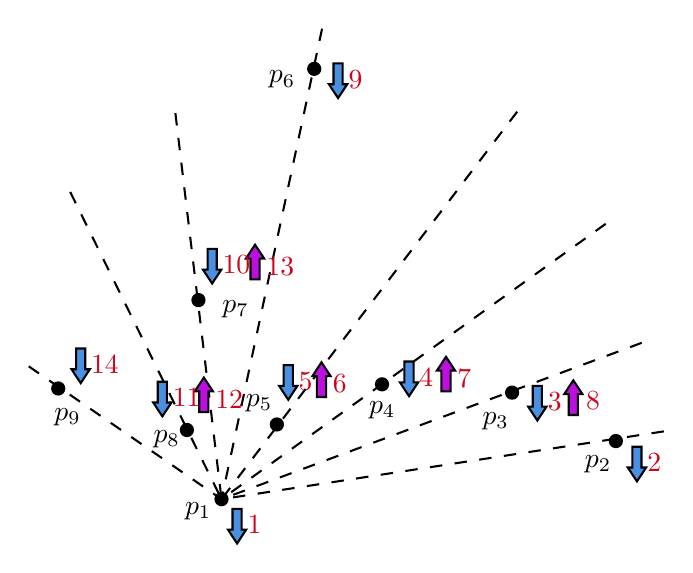
\begin{tikzpicture}[x=0.5pt,y=0.5pt,yscale=-1,xscale=1]
%uncomment if require: \path (0,384); %set diagram left start at 0, and has height of 384

%Flowchart: Connector [id:dp05090347480351787] 
\draw  [fill={rgb, 255:red, 0; green, 0; blue, 0 }  ,fill opacity=1 ] (6,263) .. controls (6,260.58) and (7.96,258.62) .. (10.38,258.62) .. controls (12.79,258.62) and (14.75,260.58) .. (14.75,263) .. controls (14.75,265.42) and (12.79,267.38) .. (10.38,267.38) .. controls (7.96,267.38) and (6,265.42) .. (6,263) -- cycle ;
%Flowchart: Connector [id:dp3291568735294871] 
\draw  [fill={rgb, 255:red, 0; green, 0; blue, 0 }  ,fill opacity=1 ] (191,32) .. controls (191,29.58) and (192.96,27.62) .. (195.38,27.62) .. controls (197.79,27.62) and (199.75,29.58) .. (199.75,32) .. controls (199.75,34.42) and (197.79,36.38) .. (195.38,36.38) .. controls (192.96,36.38) and (191,34.42) .. (191,32) -- cycle ;
%Flowchart: Connector [id:dp6621594719883535] 
\draw  [fill={rgb, 255:red, 0; green, 0; blue, 0 }  ,fill opacity=1 ] (409,301) .. controls (409,298.58) and (410.96,296.62) .. (413.38,296.62) .. controls (415.79,296.62) and (417.75,298.58) .. (417.75,301) .. controls (417.75,303.42) and (415.79,305.38) .. (413.38,305.38) .. controls (410.96,305.38) and (409,303.42) .. (409,301) -- cycle ;
%Flowchart: Connector [id:dp25920829224973985] 
\draw  [fill={rgb, 255:red, 0; green, 0; blue, 0 }  ,fill opacity=1 ] (124,343) .. controls (124,340.58) and (125.96,338.62) .. (128.38,338.62) .. controls (130.79,338.62) and (132.75,340.58) .. (132.75,343) .. controls (132.75,345.42) and (130.79,347.38) .. (128.38,347.38) .. controls (125.96,347.38) and (124,345.42) .. (124,343) -- cycle ;
%Flowchart: Connector [id:dp02220382507011076] 
\draw  [fill={rgb, 255:red, 0; green, 0; blue, 0 }  ,fill opacity=1 ] (107.33,199.13) .. controls (107.33,196.71) and (109.29,194.75) .. (111.71,194.75) .. controls (114.12,194.75) and (116.08,196.71) .. (116.08,199.13) .. controls (116.08,201.54) and (114.12,203.5) .. (111.71,203.5) .. controls (109.29,203.5) and (107.33,201.54) .. (107.33,199.13) -- cycle ;
%Flowchart: Connector [id:dp23175126343110752] 
\draw  [fill={rgb, 255:red, 0; green, 0; blue, 0 }  ,fill opacity=1 ] (164,289) .. controls (164,286.58) and (165.96,284.62) .. (168.38,284.62) .. controls (170.79,284.62) and (172.75,286.58) .. (172.75,289) .. controls (172.75,291.42) and (170.79,293.38) .. (168.38,293.38) .. controls (165.96,293.38) and (164,291.42) .. (164,289) -- cycle ;
%Flowchart: Connector [id:dp17094843613555022] 
\draw  [fill={rgb, 255:red, 0; green, 0; blue, 0 }  ,fill opacity=1 ] (99,293) .. controls (99,290.58) and (100.96,288.62) .. (103.38,288.62) .. controls (105.79,288.62) and (107.75,290.58) .. (107.75,293) .. controls (107.75,295.42) and (105.79,297.38) .. (103.38,297.38) .. controls (100.96,297.38) and (99,295.42) .. (99,293) -- cycle ;
%Flowchart: Connector [id:dp226256241933963] 
\draw  [fill={rgb, 255:red, 0; green, 0; blue, 0 }  ,fill opacity=1 ] (334,266) .. controls (334,263.58) and (335.96,261.62) .. (338.38,261.62) .. controls (340.79,261.62) and (342.75,263.58) .. (342.75,266) .. controls (342.75,268.42) and (340.79,270.38) .. (338.38,270.38) .. controls (335.96,270.38) and (334,268.42) .. (334,266) -- cycle ;
%Straight Lines [id:da8400967027516107] 
\draw  [dash pattern={on 4.5pt off 4.5pt}]  (448.04,294) -- (128.38,343) ;
%Straight Lines [id:da35176427780376085] 
\draw  [dash pattern={on 4.5pt off 4.5pt}]  (432.04,230) -- (128.38,343) ;
%Straight Lines [id:da44754220202255635] 
\draw  [dash pattern={on 4.5pt off 4.5pt}]  (201.04,3) -- (128.38,343) ;
%Straight Lines [id:da6411291076726345] 
\draw  [dash pattern={on 4.5pt off 4.5pt}]  (406.04,144) -- (128.38,343) ;
%Straight Lines [id:da7765810667431168] 
\draw  [dash pattern={on 4.5pt off 4.5pt}]  (342.04,63) -- (128.38,343) ;
%Straight Lines [id:da25629499567852587] 
\draw  [dash pattern={on 4.5pt off 4.5pt}]  (19.04,121) -- (128.38,343) ;
%Straight Lines [id:da38301578845287143] 
\draw  [dash pattern={on 4.5pt off 4.5pt}]  (95.04,64) -- (128.38,343) ;
%Straight Lines [id:da16640897796311926] 
\draw  [dash pattern={on 4.5pt off 4.5pt}]  (-10.96,247) -- (128.38,343) ;
%Flowchart: Connector [id:dp1733314058116755] 
\draw  [fill={rgb, 255:red, 0; green, 0; blue, 0 }  ,fill opacity=1 ] (240,260) .. controls (240,257.58) and (241.96,255.62) .. (244.38,255.62) .. controls (246.79,255.62) and (248.75,257.58) .. (248.75,260) .. controls (248.75,262.42) and (246.79,264.38) .. (244.38,264.38) .. controls (241.96,264.38) and (240,262.42) .. (240,260) -- cycle ;
%Down Arrow [id:dp5063296890502299] 
\draw  [fill={rgb, 255:red, 74; green, 144; blue, 226 }  ,fill opacity=1 ] (133,364.98) -- (136.31,364.98) -- (136.31,349.96) -- (142.92,349.96) -- (142.92,364.98) -- (146.23,364.98) -- (139.62,375) -- cycle ;
%Down Arrow [id:dp21678159444166145] 
\draw  [fill={rgb, 255:red, 74; green, 144; blue, 226 }  ,fill opacity=1 ] (350,276.13) -- (353.31,276.13) -- (353.31,261.11) -- (359.92,261.11) -- (359.92,276.13) -- (363.23,276.13) -- (356.62,286.15) -- cycle ;
%Down Arrow [id:dp6650103756429173] 
\draw  [fill={rgb, 255:red, 74; green, 144; blue, 226 }  ,fill opacity=1 ] (422,320.13) -- (425.31,320.13) -- (425.31,305.11) -- (431.92,305.11) -- (431.92,320.13) -- (435.23,320.13) -- (428.62,330.15) -- cycle ;
%Down Arrow [id:dp802092939622919] 
\draw  [fill={rgb, 255:red, 74; green, 144; blue, 226 }  ,fill opacity=1 ] (257.28,258.53) -- (260.59,258.53) -- (260.59,243.5) -- (267.21,243.5) -- (267.21,258.53) -- (270.51,258.53) -- (263.9,268.54) -- cycle ;
%Down Arrow [id:dp347678952148445] 
\draw  [fill={rgb, 255:red, 74; green, 144; blue, 226 }  ,fill opacity=1 ] (170,261.13) -- (173.31,261.13) -- (173.31,246.11) -- (179.92,246.11) -- (179.92,261.13) -- (183.23,261.13) -- (176.62,271.15) -- cycle ;
%Down Arrow [id:dp2571168081440359] 
\draw  [fill={rgb, 255:red, 74; green, 144; blue, 226 }  ,fill opacity=1 ] (206,43.13) -- (209.31,43.13) -- (209.31,28.11) -- (215.92,28.11) -- (215.92,43.13) -- (219.23,43.13) -- (212.62,53.15) -- cycle ;
%Down Arrow [id:dp43517140651566777] 
\draw  [fill={rgb, 255:red, 74; green, 144; blue, 226 }  ,fill opacity=1 ] (115,177.13) -- (118.31,177.13) -- (118.31,162.11) -- (124.92,162.11) -- (124.92,177.13) -- (128.23,177.13) -- (121.62,187.15) -- cycle ;
%Down Arrow [id:dp31131733900650227] 
\draw  [fill={rgb, 255:red, 74; green, 144; blue, 226 }  ,fill opacity=1 ] (79,273.13) -- (82.31,273.13) -- (82.31,258.11) -- (88.92,258.11) -- (88.92,273.13) -- (92.23,273.13) -- (85.62,283.15) -- cycle ;
%Down Arrow [id:dp9776785564723787] 
\draw  [fill={rgb, 255:red, 74; green, 144; blue, 226 }  ,fill opacity=1 ] (20,249.13) -- (23.31,249.13) -- (23.31,234.11) -- (29.92,234.11) -- (29.92,249.13) -- (33.23,249.13) -- (26.62,259.15) -- cycle ;
%Down Arrow [id:dp6804288828832812] 
\draw  [fill={rgb, 255:red, 189; green, 16; blue, 224 }  ,fill opacity=1 ] (207.23,254.12) -- (203.92,254.12) -- (203.92,269.15) -- (197.31,269.15) -- (197.31,254.12) -- (194,254.12) -- (200.62,244.11) -- cycle ;
%Down Arrow [id:dp2744672671561321] 
\draw  [fill={rgb, 255:red, 189; green, 16; blue, 224 }  ,fill opacity=1 ] (297.23,250.12) -- (293.92,250.12) -- (293.92,265.15) -- (287.31,265.15) -- (287.31,250.12) -- (284,250.12) -- (290.62,240.11) -- cycle ;
%Down Arrow [id:dp749364135043204] 
\draw  [fill={rgb, 255:red, 189; green, 16; blue, 224 }  ,fill opacity=1 ] (389.23,267.12) -- (385.92,267.12) -- (385.92,282.15) -- (379.31,282.15) -- (379.31,267.12) -- (376,267.12) -- (382.62,257.11) -- cycle ;
%Down Arrow [id:dp4501075590171838] 
\draw  [fill={rgb, 255:red, 189; green, 16; blue, 224 }  ,fill opacity=1 ] (159.23,169.12) -- (155.92,169.12) -- (155.92,184.15) -- (149.31,184.15) -- (149.31,169.12) -- (146,169.12) -- (152.62,159.11) -- cycle ;
%Down Arrow [id:dp720924322469968] 
\draw  [fill={rgb, 255:red, 189; green, 16; blue, 224 }  ,fill opacity=1 ] (122.23,265.12) -- (118.92,265.12) -- (118.92,280.15) -- (112.31,280.15) -- (112.31,265.12) -- (109,265.12) -- (115.62,255.11) -- cycle ;

% Text Node
\draw (77,290.93) node [anchor=north west][inner sep=0.75pt]   [align=left] {$\displaystyle p_{8}$};
% Text Node
\draw (126.75,196.93) node [anchor=north west][inner sep=0.75pt]   [align=left] {$\displaystyle p_{7}$};
% Text Node
\draw (143.75,264.93) node [anchor=north west][inner sep=0.75pt]   [align=left] {$\displaystyle p_{5}$};
% Text Node
\draw (232.75,269.93) node [anchor=north west][inner sep=0.75pt]   [align=left] {$\displaystyle p_{4}$};
% Text Node
\draw (99.75,342.93) node [anchor=north west][inner sep=0.75pt]   [align=left] {$\displaystyle p_{1}$};
% Text Node
\draw (388.75,308.93) node [anchor=north west][inner sep=0.75pt]   [align=left] {$\displaystyle p_{2}$};
% Text Node
\draw (5.38,275.31) node [anchor=north west][inner sep=0.75pt]   [align=left] {$\displaystyle p_{9}$};
% Text Node
\draw (160.38,31.31) node [anchor=north west][inner sep=0.75pt]   [align=left] {$\displaystyle p_{6}$};
% Text Node
\draw (314.75,277.93) node [anchor=north west][inner sep=0.75pt]   [align=left] {$\displaystyle p_{3}$};
% Text Node
\draw (144.92,352.89) node [anchor=north west][inner sep=0.75pt]   [align=left] {\textcolor[rgb]{0.82,0.01,0.11}{1}};
% Text Node
\draw (433.92,308.04) node [anchor=north west][inner sep=0.75pt]   [align=left] {$\displaystyle \textcolor[rgb]{0.82,0.01,0.11}{2}$};
% Text Node
\draw (361.92,264.04) node [anchor=north west][inner sep=0.75pt]   [align=left] {$\displaystyle \textcolor[rgb]{0.82,0.01,0.11}{3}$};
% Text Node
\draw (269.21,246.44) node [anchor=north west][inner sep=0.75pt]   [align=left] {$\displaystyle \textcolor[rgb]{0.82,0.01,0.11}{4}$};
% Text Node
\draw (181.92,249.04) node [anchor=north west][inner sep=0.75pt]   [align=left] {$\displaystyle \textcolor[rgb]{0.82,0.01,0.11}{5}$};
% Text Node
\draw (217.92,31.04) node [anchor=north west][inner sep=0.75pt]   [align=left] {$\displaystyle \textcolor[rgb]{0.82,0.01,0.11}{9}$};
% Text Node
\draw (206.62,251.04) node [anchor=north west][inner sep=0.75pt]   [align=left] {$\displaystyle \textcolor[rgb]{0.82,0.01,0.11}{6}$};
% Text Node
\draw (296.62,247.04) node [anchor=north west][inner sep=0.75pt]   [align=left] {$\displaystyle \textcolor[rgb]{0.82,0.01,0.11}{7}$};
% Text Node
\draw (389.62,263.04) node [anchor=north west][inner sep=0.75pt]   [align=left] {$\displaystyle \textcolor[rgb]{0.82,0.01,0.11}{8}$};
% Text Node
\draw (158.62,166.04) node [anchor=north west][inner sep=0.75pt]   [align=left] {$\displaystyle \textcolor[rgb]{0.82,0.01,0.11}{13}$};
% Text Node
\draw (90.92,261.04) node [anchor=north west][inner sep=0.75pt]   [align=left] {$\displaystyle \textcolor[rgb]{0.82,0.01,0.11}{11}$};
% Text Node
\draw (121.62,262.04) node [anchor=north west][inner sep=0.75pt]   [align=left] {$\displaystyle \textcolor[rgb]{0.82,0.01,0.11}{12}$};
% Text Node
\draw (126.92,165.04) node [anchor=north west][inner sep=0.75pt]   [align=left] {$\displaystyle \textcolor[rgb]{0.82,0.01,0.11}{10}$};
% Text Node
\draw (31.92,237.04) node [anchor=north west][inner sep=0.75pt]   [align=left] {$\displaystyle \textcolor[rgb]{0.82,0.01,0.11}{14}$};


\end{tikzpicture}

